\documentclass[17pt, orivec]{extarticle} % 12pt, 14pt, 17pt, 20pt
\usepackage{amsmath}
\usepackage{amssymb}    % for \rightsquigarrow
\usepackage{wasysym}	% for frown face
\usepackage{mathrsfs} 	% for \mathscr
\usepackage{stmaryrd}
\usepackage[most]{tcolorbox}
\usepackage{ulem}
\usepackage{tikz-cd}		% commutative diagrams
\usepackage{tikz}
\usepackage{amsthm}
\usepackage{enumitem}	% for \itemize custom labels
\usepackage{turnstile}	% longer turnstiles
\usepackage[sf,bf,big,raggedright,compact]{titlesec}	% change section color to blue
% \usepackage[backend=biber,bibstyle=authoryear,citestyle=../authoryearbrack]{biblatex}
% \bibliography{../AGI-book}

\newtheorem{theorem}{Theorem}

\ifdefined\chinchin
	\newcommand{\cc}[2]{#1}
	\usepackage[CJKspace]{xeCJK}
	%\setCJKmainfont[BoldFont=SimHei,ItalicFont=AR PL KaitiM GB]{Alibaba PuHuiTi}
	\setCJKmainfont[BoldFont=Alibaba-PuHuiTi-Regular.ttf, ItalicFont=gkai00mp.ttf]{Alibaba-PuHuiTi-Light.ttf}
	% \setmainfont[ItalicFont=Latin Modern Roman Slanted]{Alibaba Sans:style=Light}
\else
	\newcommand{\cc}[2]{#2}
	% \setmainfont[ItalicFont=Latin Modern Roman Slanted]{Alibaba Sans:style=Light}
	%\renewcommand{\baselinestretch}{0.8} 
\fi

%\ifdefined\chinchin
%\newcommand{\cc}[2]{#1}
%\usepackage[CJKspace]{xeCJK}
%\setCJKmainfont[BoldFont=SimHei,ItalicFont=AR PL KaitiM GB]{SimSun}
%\else
%\newcommand{\cc}[2]{#2}
%\fi

\setlength{\headheight}{0cm}
\setlength{\hoffset}{0cm}
\setlength{\topmargin}{-2cm}
\setlength{\oddsidemargin}{-2cm}
\setlength{\evensidemargin}{-2cm}
\setlength{\textwidth}{20cm}
\setlength{\textheight}{26cm}
\setlength{\headsep}{0cm}
\setlength{\topskip}{0cm}
\setlength{\footskip}{0.9cm}  % between bottom of page and page number
\setlength{\floatsep}{0cm}
\setlength{\textfloatsep}{0.6cm}
\setlength{\intextsep}{0.5cm}
\setlength{\parindent}{0em}   % em = width of capital M

% Fix spilling of titles in bibliography:
%\DeclareFieldFormat*{title}{#1}
%
%\DeclareFieldFormat*{titlecase}{%
%    \ifdef{\currentfield}
%      {\ifcurrentfield{title}
%         {\usefield{\uline}{\currentfield}}%
%         {#1}}
%      {#1}}

\setcounter{secnumdepth}{2}		% no section numbers

\titleformat{\section}[hang]{\bfseries\Large\color{blue}}{\thesection \hspace{20pt}}{0pt}{}
\titleformat{\subsection}[hang]{\bfseries\large\color{blue}}{\thesubsection \hspace{10pt}}{0pt}{}
\titleformat{\subsubsection}[hang]{\bfseries\color{blue}}{}{0pt}{}

\itemsep0em
\setlist[itemize]{noitemsep, topsep=-5pt, partopsep=-5pt}
\renewcommand{\labelitemi}{$\textbullet$}

\let\varzero\emptyset
\let\emptyset\varnothing		% round empty set 
\newcommand{\vect}[1]{\boldsymbol{#1}}
\newcommand{\book}[1]{$\NewSym[0.4]{../book-icon.png} \quad$ \parbox{0.9\textwidth}{\footnotesize #1}}
\newcommand{\code}[1]{{\footnotesize{\ttfamily #1}}}
\newcommand{\tab}{\hspace*{2cm}}
\newcommand{\powerset}{\raisebox{.15\baselineskip}{\Large\ensuremath{\wp}}}
\newcommand{\Chi}{\raisebox{2.5pt}{$\chi$}}
\newcommand*\KB{\vcenter{\hbox{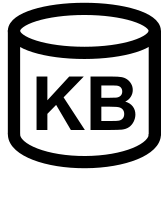
\includegraphics{../KB-symbol.png}}}}
\newcommand*\NewSym[2][0.5]{\vcenter{\hbox{\includegraphics[scale=#1]{#2}}}}
\newcommand*\sigmoid{\vcenter{\hbox{
\includegraphics{../sigmoid3.png}}}}
\newcommand{\smbox}[1]{\boxed{\footnotesize{\mbox{#1}}}}

\newcommand{\tikzmark}[1]{\tikz[overlay,remember picture] \node (#1) {};}

\newcommand{\Dfrac}[2]{%
\ooalign{%
      $\genfrac{}{}{2.9pt}0{\hphantom{#1}}{\hphantom{#2}}$\cr%
      $\color{white}\genfrac{}{}{1.5pt}0{\hphantom{#1}}{\hphantom{#2}}$\cr%
      $\color{white}\genfrac{}{}{1pt}0{\color{black}#1}{\color{black}#2}$}}

% \renewcommand{\thefootnote}{\fnsymbol{footnote}}
\usepackage{perpage}
\MakePerPage{footnote}
\renewcommand{\thefootnote}{\ifcase\value{footnote}\or{*}
	\or{$\dagger$}\or{**}\or{$\ddagger$}\fi}
\interfootnotelinepenalty=10000

\setlength{\parindent}{0pt}
\setlength{\parskip}{1.8ex plus0.8ex minus0.8ex}

% \usepackage[no-math]{fontspec}
% \setmainfont[BoldFont=Alibaba_Sans_Regular.otf,ItalicFont=Alibaba_Sans_Light_Italic.otf]{Alibaba_Sans_Light.otf}

\usepackage[backend=biber]{biblatex}
\bibliography{../AGI-book}

\usepackage[active,tightpage]{preview}		% for continuous page(s)
\renewcommand{\PreviewBorder}{0.5cm}
\renewcommand{\thempfootnote}{\arabic{mpfootnote}}

\usepackage[absolute,overlay]{textpos}		% for page number on upper left corner

\usepackage{color}
% \usepackage{mathtools}
\usepackage[hyperfootnotes=false]{hyperref}

% \usepackage[backend=biber,style=numeric]{biblatex}
% \bibliography{../AGI-book}
% \renewcommand*{\bibfont}{\footnotesize}

\usetikzlibrary{shapes}
% \usepackage[export]{adjustbox}	% ??
\usepackage{verbatim} % for comments
% \usepackage{newtxtext,newtxmath}	% Times New Roman font

% \titleformat{\subsection}[hang]{\bfseries\large\color{blue}}{}{0pt}{} 
% \numberwithin{equation}{subsection}

\newcommand{\underdash}[1]{%
	\tikz[baseline=(toUnderline.base)]{
		\node[inner sep=1pt,outer sep=10pt] (toUnderline) {#1};
		\draw[dashed] ([yshift=-0pt]toUnderline.south west) -- ([yshift=-0pt]toUnderline.south east);
	}%
}%

\newcommand\reduline{\bgroup\markoverwith{\textcolor{red}{\rule[-0.5ex]{2pt}{0.4pt}}}\ULon}

%\DeclareSymbolFont{symbolsC}{U}{txsyc}{m}{n}
%\DeclareMathSymbol{\strictif}{\mathrel}{symbolsC}{74}
%\DeclareSymbolFont{AMSb}{U}{msb}{m}{n}
%\DeclareSymbolFontAlphabet{\mathbb}{AMSb}
%\setmathfont{lmroman17-regular.otf}
\DeclareMathOperator*{\argmin}{arg\,min}
\DeclareMathOperator*{\argmax}{arg\,max}

% \usepackage[most]{tcolorbox}
%\tcbset{on line, 
%	boxsep=4pt, left=0pt,right=0pt,top=0pt,bottom=0pt,
%	colframe=red,colback=pink,
%	highlight math style={enhanced}
%}
%\newcommand{\atom}{\vcenter{\hbox{\tcbox{....}}}}

\let\oldtextbf\textbf
\renewcommand{\textbf}[1]{\textcolor{blue}{\oldtextbf{#1}}}

\newcommand{\logic}[1]{{\color{violet}{\textit{#1}}}}
\newcommand{\underconst}{
\includegraphics[scale=0.5]{../2020/UnderConst.png}}
\newcommand{\KBsymbol}{\vcenter{\hbox{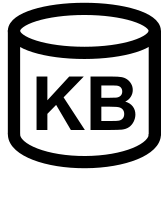
\includegraphics[scale=1]{../KB-symbol.png}}}}
\newcommand{\token}{\vcenter{\hbox{\includegraphics[scale=1]{token.png}}}}
\newcommand{\proposition}{\vcenter{\hbox{\includegraphics[scale=0.8]{proposition.png}}}}

\begin{document}

\begin{preview}

\title{\vspace{-1.5cm} \bfseries\color{blue}{\LARGE \cc{什么是落后?}{What is backwardness?}}}

% \author{YKY} % Your name
\date{\vspace{-2.4cm} \tiny \today} % Date, can be changed to a custom date

\maketitle

\setcounter{section}{-1}
\newcounter{mypage}
\setcounter{mypage}{0}

\begin{minipage}{\textwidth}
\setlength{\parskip}{0.4\baselineskip}
\begin{textblock*}{5cm}(2.1cm,2.3cm) % {block width} (coords) 
	{\color{red}{\large \textcircled{\small \themypage}}}
	\addtocounter{mypage}{1}
\end{textblock*}

\begin{itemize}
	\item \cc{落后 并不是一种有形体的物质,而是 \textbf{进步思想的缺如};\\
		别人进步了,而你停滞不前,就会落后}
		{}
	\item \cc{在 西藏 未被中国共产党解放之前,他们仍然有很原始的习俗,\\
		例如将 16岁 少女活剥人皮,制成所谓吉祥物}
		{}
	\begin{equation}
		\vcenter{\hbox{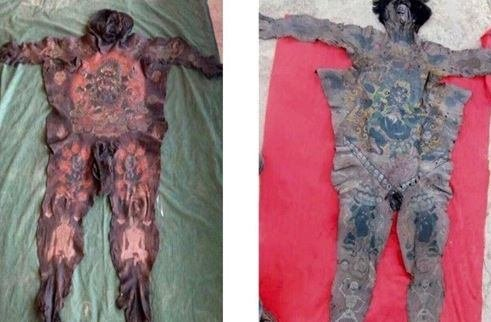
\includegraphics[scale=0.7]{Tibet-human-skin.jpg}}}
		\nonumber
	\end{equation}
		\cc{如果没有 \textbf{外来的} 力量影响,他们很可能会继续这些野蛮传统}
		{}
	\item 有些人民明知制度是残酷的,但不敢反抗,\\
		也有人会利用制度,陷害他们所妒忌的人 
		\footnote{在 西门豹治邺 的故事里(历史记载他是战国时代的人,是否真有其事并不影响我的论点),村民其实知道 河伯娶妻 = 送死,他们被送去见河伯时叩头求饶}
	\item 「落后」可以用科学的方法 \textbf{量度},\\
		它是人民的思想(或意识形态)与 \textbf{真实} 之间的距离 \\
		落后国家人民普遍 迷信,浪费能量和资源、降低效率、导致贫困
	\item 例如,在 \textbf{伊斯兰} 原教旨主义下,妇女必需包头、不可读书或驾车\\
		对妇女的压抑 导致一半人口失去经济竞争力
	\item Malala 在 16岁那年上学途中 遭 塔利班 恐怖分子 枪击,但侥幸生还 \\
		她现在移民到美国 从事人道主义工作 \\
		\begin{equation}
		\vcenter{\hbox{
\includegraphics[scale=0.2]{Malala.jpg}}}
		\nonumber
		\end{equation}
\end{itemize}

\end{minipage}
\end{preview}

\begin{preview}
\begin{textblock*}{5cm}(2.1cm,2.3cm) % {block width} (coords) 
	{\color{red}{\large \textcircled{\small \themypage}}}
	\addtocounter{mypage}{1}
\end{textblock*}
\begin{minipage}{\textwidth}
	\setlength{\parskip}{0.4\baselineskip}

\section{Jared Diamond 的 地理决定论}

\begin{itemize}
	\item 人类 (homo sapiens) 起源于非洲的人猿 (primates),\\
		继而散布到其他大陆 \\
	\begin{equation}
	\vcenter{\hbox{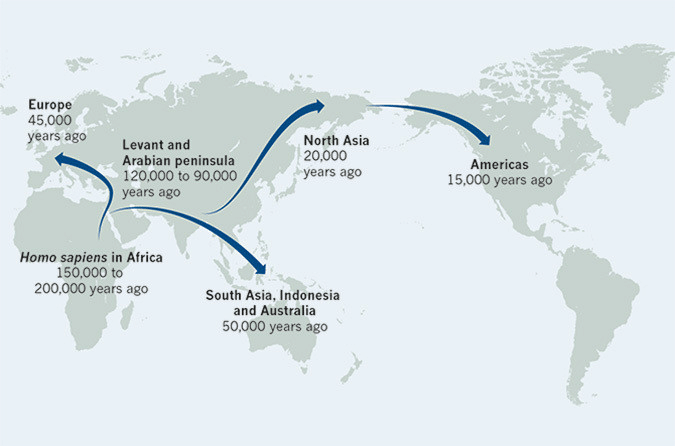
\includegraphics[scale=1]{homo-sapiens-migration.png}}}
	\nonumber
	\end{equation}
	\item 一个欧洲白人\footnote{她是影星 Ingrid Bergman, Jared Diamond 选的例子} 跟一个 新几内亚 土著 比较,\\
		她的种族并不比他的「更年轻」,两个种族在同一时间轴上同时进化
		\begin{equation}
		\vcenter{\hbox{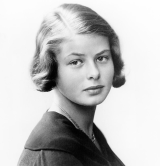
\includegraphics[scale=1]{Ingrid-Bergman.png}}}
		\qquad
		\vcenter{\hbox{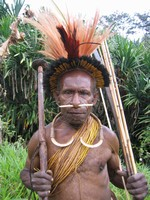
\includegraphics[scale=1]{New-Guinea-tribesman.png}}}
		\nonumber
		\end{equation}
	\item 白种人并非较为「年轻」,这是一种错觉。但白人比较「进步」\\
		为什么有些民族 较进步,有些较落后呢? \\
		著名的「\textbf{李约瑟难题}」:为什么古代中国文化那么辉煌,\\
		\tab 却没有产生出西方的科技和工业革命? \\
		Jared Diamond 的书《\textbf{枪、细菌、钢铁}》给出了答案:\textbf{地理决定论} \\
		\begin{equation}
		\vcenter{\hbox{
\includegraphics[scale=0.4]{guns-germs-steel(cover).jpg}}}
		\nonumber
		\end{equation}
	\item 偏僻的地方资讯不发达,而资讯发达的地方越来越进步 \\
		正如城市的孩子较早熟、``smart'',乡下的孩子较笨
	\item 人类文明产生于 欧亚大陆,因为那是最大的 \textbf{连通板块} \\
		而 新几内亚 是相对 \textbf{孤立} 的岛屿 \\
		在孤立的岛上,生物 (或技术) \textbf{进化的速度} 较慢
	\item 中国人并不蠢,但中国处于欧亚大陆的 \textbf{边缘} 位置 \\
		并且被山脉分隔,导致 欧亚大陆的文明 较难 传到中国
\end{itemize}

\end{minipage}
\end{preview}

\begin{preview}
\begin{textblock*}{5cm}(2.1cm,2.3cm) % {block width} (coords) 
	{\color{red}{\large \textcircled{\small \themypage}}}
	\addtocounter{mypage}{1}
\end{textblock*}
	
\begin{minipage}{\textwidth}
\setlength{\parskip}{0.4\baselineskip}

\section{贫困的原因,是 资源短缺 还是 思想落后?}

\begin{itemize}
	\item Max Weber 提出「人的 \textbf{思想} 决定社会的进步程度」\\
		他的著作《新教伦理与资本主义精神》指出天主教的腐败 \\
		基督教新教 (Protestant) 强调 人与神的直接关系 \\
		提倡个人诠释《圣经》,而不是经由 神职人员 \\
		所以在新教国家里,新的 \textbf{工作伦理} (work ethics) 令人更勤奋

	\item 马克思 则认为,\textbf{经济条件} 决定人的思想
		所以 统治阶级 继续 剥削、工人阶级 继续 愚昧
	

	\item 但有另一个问题:为什么非洲现在那么落后? \\
	为什么埃及是古文明,现在那么贫困? \\
	似乎有个现象: 文明的兴衰 就像火柴的燃烧 \\
	是 \textbf{不可逆过程}; 火柴不能燃烧两次
	\item 但需要解释: 确切是什么限制了文明是不可逆过程? \\
	是因为人耗尽了地上的资源?\\
	还是因为古文明在群体意识里,变成了历史包袱?
	\item 我认为是后者:是 意识形态 决定了落后。\\
	历史上,犹太人 经历了长达数千年的 diaspora,\\
	近代犹太人在以色列复国,其成为强大的国家,\\
	这显然不是因为土地资源决定的,\\
	而是因为 犹太人 学习了欧洲进步的文明

\end{itemize}
		
\end{minipage}
\end{preview}

\begin{comment}
\begin{preview}
\begin{textblock*}{5cm}(2.1cm,2.3cm) % {block width} (coords) 
	{\color{red}{\large \textcircled{\small \themypage}}}
	\addtocounter{mypage}{1}
\end{textblock*}

\begin{minipage}{\textwidth}
\setlength{\parskip}{0.4\baselineskip}

\section{This}

\begin{itemize}
	\item Here
\end{itemize}

\end{minipage}
\end{preview}

\end{comment}

\end{document}
